\documentclass{standalone}
\usepackage{tikz}
\usetikzlibrary{patterns}
\usetikzlibrary{positioning}
\usetikzlibrary{patterns, positioning}
\usetikzlibrary{shapes.misc}
\usepackage[outline]{contour}
\contourlength{1.5pt} 
\usepackage[sfdefault]{ClearSans}

\begin{document}
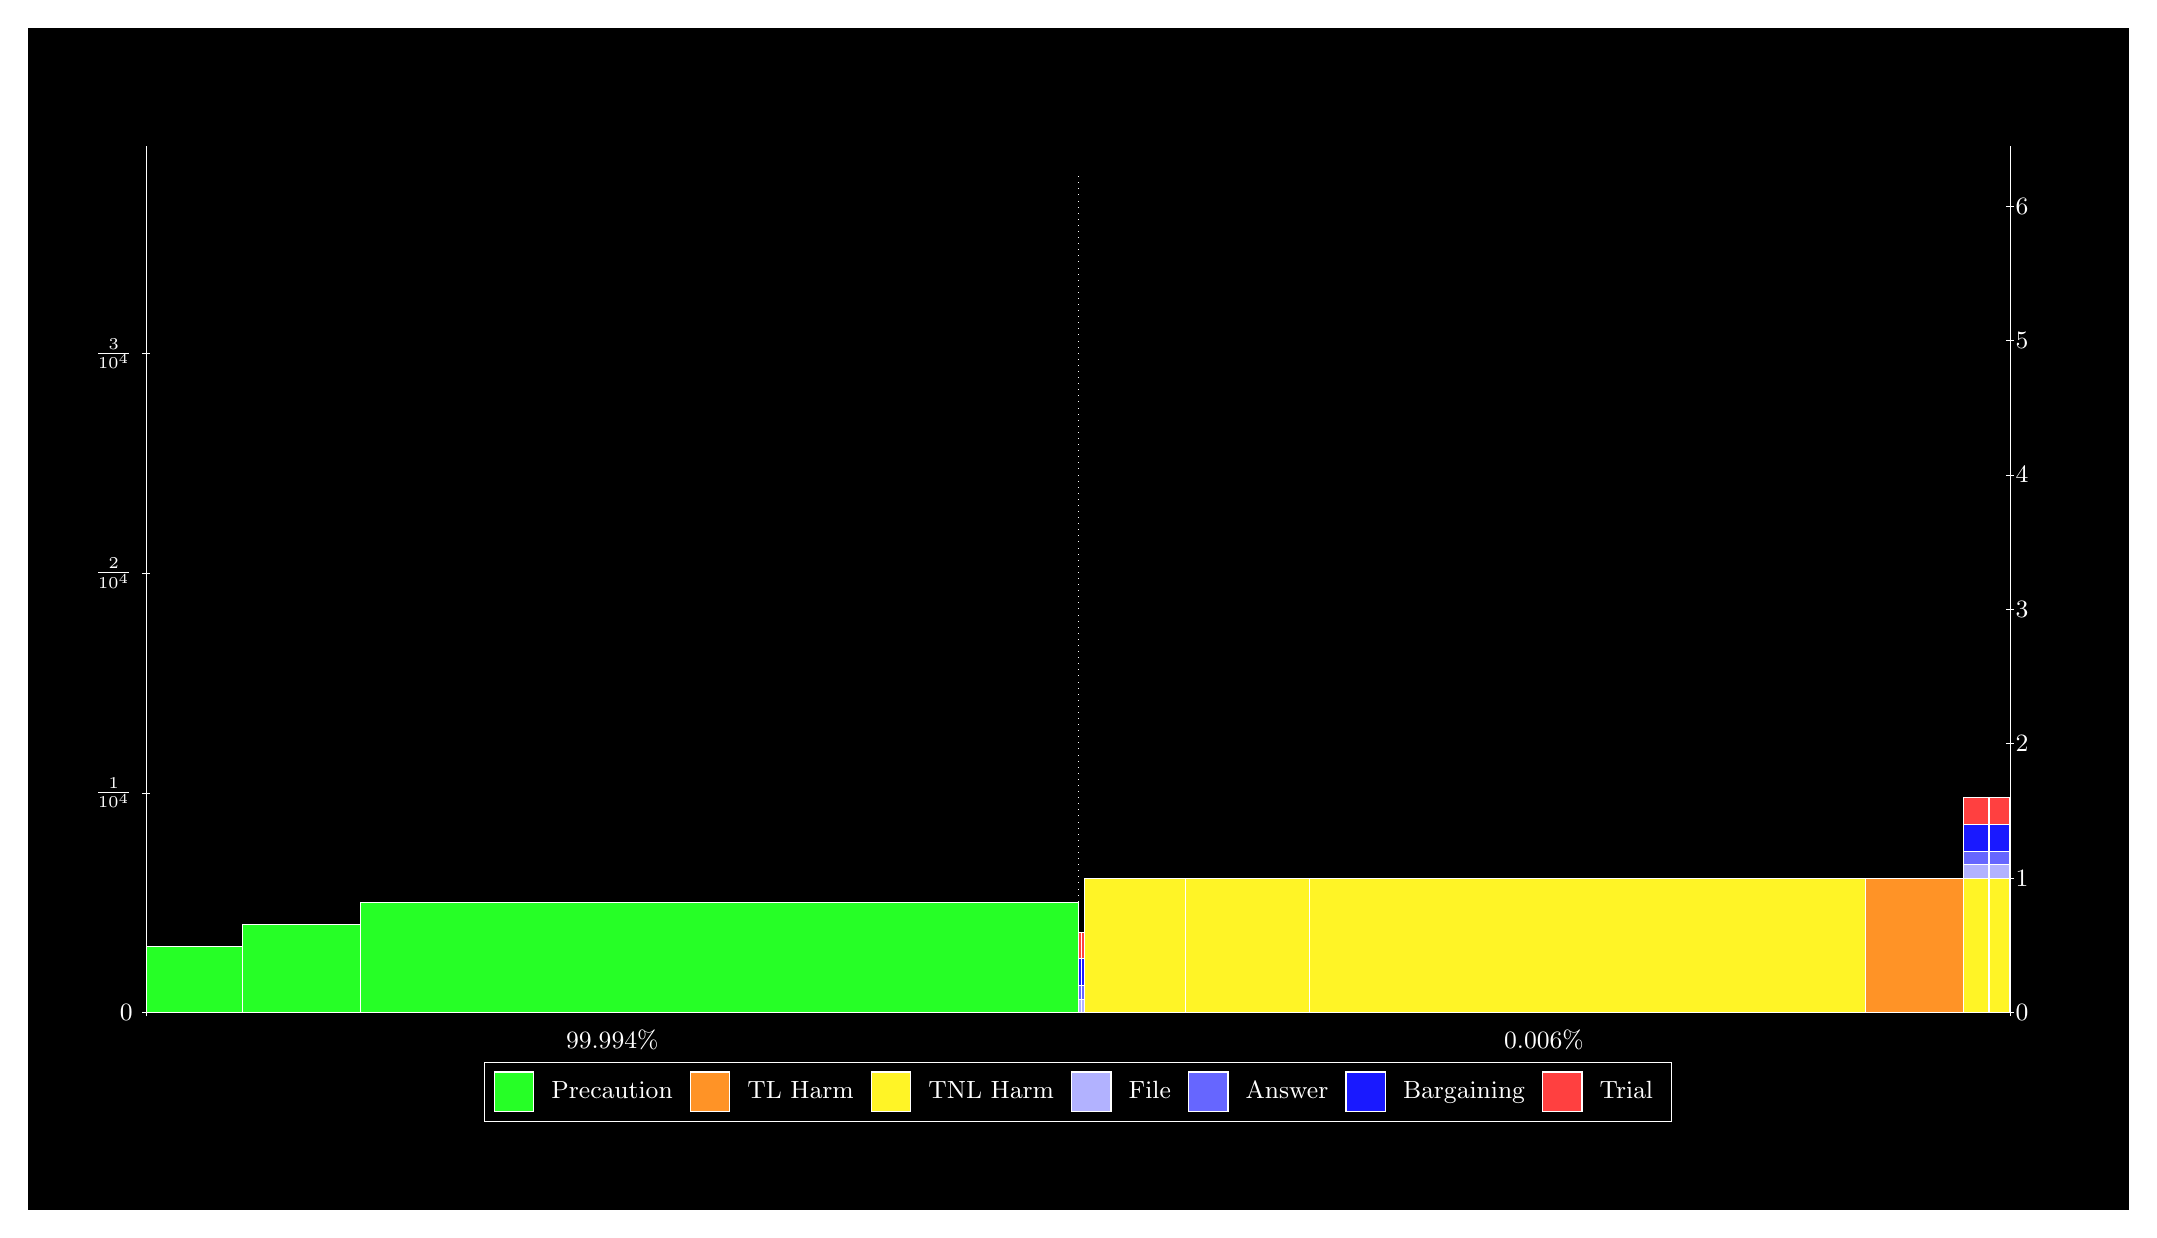
\begin{tikzpicture}
\draw[fill=black] (0,0) rectangle (26.667,15);
\draw[fill=green!85,draw=white,very thin] (1.5,2.5) rectangle (2.7168,3.3369);
\draw[fill=green!85,draw=white,very thin] (2.7168,2.5) rectangle (4.2218,3.6159);
\draw[fill=green!85,draw=white,very thin] (4.2218,2.5) rectangle (13.333,3.8948);
\draw[fill=green!85,draw=white,very thin] (13.333,2.5) rectangle (13.376,2.5001);
\draw[fill=blue!30,draw=white,very thin] (13.333,2.5001) rectangle (13.376,2.6707);
\draw[fill=blue!60,draw=white,very thin] (13.333,2.6707) rectangle (13.376,2.8414);
\draw[fill=blue!90,draw=white,very thin] (13.333,2.8414) rectangle (13.376,3.1827);
\draw[fill=red!75,draw=white,very thin] (13.333,3.1827) rectangle (13.376,3.524);
\draw[fill=green!85,draw=white,very thin] (13.376,2.5) rectangle (13.413,2.5001);
\draw[fill=blue!30,draw=white,very thin] (13.376,2.5001) rectangle (13.413,2.6707);
\draw[fill=blue!60,draw=white,very thin] (13.376,2.6707) rectangle (13.413,2.8414);
\draw[fill=blue!90,draw=white,very thin] (13.376,2.8414) rectangle (13.413,3.1827);
\draw[fill=red!75,draw=white,very thin] (13.376,3.1827) rectangle (13.413,3.5241);
\draw[fill=green!85,draw=white,very thin] (13.413,2.5) rectangle (14.688,2.5001);
\draw[fill=yellow!85,draw=white,very thin] (13.413,2.5001) rectangle (14.688,4.2067);
\draw[fill=green!85,draw=white,very thin] (14.688,2.5) rectangle (14.69,2.5001);
\draw[fill=orange!85,draw=white,very thin] (14.688,2.5001) rectangle (14.69,4.2067);
\draw[fill=green!85,draw=white,very thin] (14.69,2.5) rectangle (16.264,2.5001);
\draw[fill=yellow!85,draw=white,very thin] (14.69,2.5001) rectangle (16.264,4.2067);
\draw[fill=green!85,draw=white,very thin] (16.264,2.5) rectangle (23.33,2.5001);
\draw[fill=yellow!85,draw=white,very thin] (16.264,2.5001) rectangle (23.33,4.2067);
\draw[fill=green!85,draw=white,very thin] (23.33,2.5) rectangle (24.576,2.5001);
\draw[fill=orange!85,draw=white,very thin] (23.33,2.5001) rectangle (24.576,4.2067);
\draw[fill=green!85,draw=white,very thin] (24.576,2.5) rectangle (24.891,2.5001);
\draw[fill=yellow!85,draw=white,very thin] (24.576,2.5001) rectangle (24.891,4.2067);
\draw[fill=blue!30,draw=white,very thin] (24.576,4.2067) rectangle (24.891,4.3774);
\draw[fill=blue!60,draw=white,very thin] (24.576,4.3774) rectangle (24.891,4.548);
\draw[fill=blue!90,draw=white,very thin] (24.576,4.548) rectangle (24.891,4.8893);
\draw[fill=red!75,draw=white,very thin] (24.576,4.8893) rectangle (24.891,5.2307);
\draw[fill=green!85,draw=white,very thin] (24.891,2.5) rectangle (24.911,2.5001);
\draw[fill=orange!85,draw=white,very thin] (24.891,2.5001) rectangle (24.911,4.2067);
\draw[fill=blue!30,draw=white,very thin] (24.891,4.2067) rectangle (24.911,4.3774);
\draw[fill=blue!60,draw=white,very thin] (24.891,4.3774) rectangle (24.911,4.548);
\draw[fill=blue!90,draw=white,very thin] (24.891,4.548) rectangle (24.911,4.8893);
\draw[fill=red!75,draw=white,very thin] (24.891,4.8893) rectangle (24.911,5.2307);
\draw[fill=green!85,draw=white,very thin] (24.911,2.5) rectangle (25.163,2.5001);
\draw[fill=yellow!85,draw=white,very thin] (24.911,2.5001) rectangle (25.163,4.2067);
\draw[fill=blue!30,draw=white,very thin] (24.911,4.2067) rectangle (25.163,4.3774);
\draw[fill=blue!60,draw=white,very thin] (24.911,4.3774) rectangle (25.163,4.548);
\draw[fill=blue!90,draw=white,very thin] (24.911,4.548) rectangle (25.163,4.8894);
\draw[fill=red!75,draw=white,very thin] (24.911,4.8894) rectangle (25.163,5.2307);
\draw[fill=green!85,draw=white,very thin] (25.163,2.5) rectangle (25.167,2.5001);
\draw[fill=orange!85,draw=white,very thin] (25.163,2.5001) rectangle (25.167,4.2067);
\draw[fill=blue!30,draw=white,very thin] (25.163,4.2067) rectangle (25.167,4.3774);
\draw[fill=blue!60,draw=white,very thin] (25.163,4.3774) rectangle (25.167,4.548);
\draw[fill=blue!90,draw=white,very thin] (25.163,4.548) rectangle (25.167,4.8894);
\draw[fill=red!75,draw=white,very thin] (25.163,4.8894) rectangle (25.167,5.2307);
\draw[white,very thin] (1.5,2.5) -- (1.5,13.5);
\draw[white,very thin] (1.45,2.5) -- (1.55,2.5);
\node[font=\small,text=white, anchor=east] at (1.45, 2.5) {0};
\draw[white,very thin] (1.45,5.2897) -- (1.55,5.2897);
\node[font=\small,text=white, anchor=east] at (1.45, 5.2897) {$\frac{1}{10^{4}}$};
\draw[white,very thin] (1.45,8.0794) -- (1.55,8.0794);
\node[font=\small,text=white, anchor=east] at (1.45, 8.0794) {$\frac{2}{10^{4}}$};
\draw[white,very thin] (1.45,10.869) -- (1.55,10.869);
\node[font=\small,text=white, anchor=east] at (1.45, 10.869) {$\frac{3}{10^{4}}$};

\draw[white,dotted,very thin] (13.333,2.83) -- (13.333,13.17);
\draw[white,very thin] (25.167,2.5) -- (25.167,13.5);
\draw[white,very thin] (25.117,2.5) -- (25.217,2.5);
\node[font=\small,text=white, anchor=west] at (25.117, 2.5) {0};
\draw[white,very thin] (25.117,4.2066) -- (25.217,4.2066);
\node[font=\small,text=white, anchor=west] at (25.117, 4.2066) {1};
\draw[white,very thin] (25.117,5.9133) -- (25.217,5.9133);
\node[font=\small,text=white, anchor=west] at (25.117, 5.9133) {2};
\draw[white,very thin] (25.117,7.6199) -- (25.217,7.6199);
\node[font=\small,text=white, anchor=west] at (25.117, 7.6199) {3};
\draw[white,very thin] (25.117,9.3266) -- (25.217,9.3266);
\node[font=\small,text=white, anchor=west] at (25.117, 9.3266) {4};
\draw[white,very thin] (25.117,11.033) -- (25.217,11.033);
\node[font=\small,text=white, anchor=west] at (25.117, 11.033) {5};
\draw[white,very thin] (25.117,12.74) -- (25.217,12.74);
\node[font=\small,text=white, anchor=west] at (25.117, 12.74) {6};

\draw[white,very thin] (1.5,2.5) -- (25.167,2.5);
\draw[white,very thin] (1.5,2.45) -- (1.5,2.55);
\node[font=\small,text=white, anchor=north] at (1.5, 2.45) {};
\draw[white,very thin] (25.167,2.45) -- (25.167,2.55);
\node[font=\small,text=white, anchor=north] at (25.167, 2.45) {};

\node[font=\small,text=white,anchor=south] at (7.4167, 1.9) {99.994\%};
\node[font=\small,text=white,anchor=south] at (19.25, 1.9) {0.006\%};
\draw (13.3333,2.5) node (B) {};
\begin{scope}[align=center]
\matrix[scale=0.5,draw=white,below=0.5cm of B,nodes={draw},column sep=0.1cm]{
\node[rectangle,draw,minimum width=0.5cm,minimum height=0.5cm,fill=green!85]{}; & \node[draw=none,font=\small,text=white]{Precaution}; &
\node[rectangle,draw,minimum width=0.5cm,minimum height=0.5cm,fill=orange!85]{}; & \node[draw=none,font=\small,text=white]{TL Harm}; &
\node[rectangle,draw,minimum width=0.5cm,minimum height=0.5cm,fill=yellow!85]{}; & \node[draw=none,font=\small,text=white]{TNL Harm}; &
\node[rectangle,draw,minimum width=0.5cm,minimum height=0.5cm,fill=blue!30]{}; & \node[draw=none,font=\small,text=white]{File}; &
\node[rectangle,draw,minimum width=0.5cm,minimum height=0.5cm,fill=blue!60]{}; & \node[draw=none,font=\small,text=white]{Answer}; &
\node[rectangle,draw,minimum width=0.5cm,minimum height=0.5cm,fill=blue!90]{}; & \node[draw=none,font=\small,text=white]{Bargaining}; &
\node[rectangle,draw,minimum width=0.5cm,minimum height=0.5cm,fill=red!75]{}; & \node[draw=none,font=\small,text=white]{Trial}; \\\\
};\end{scope}

\end{tikzpicture}
\end{document}